\chapter{DEEP LEARNING AND DEEP NEURAL NETWORKS}
\thispagestyle{fancy}

	In recent years, the popularity of deep learning has increased enormously in the machine learning
community. Deep learning tries to model and extract high-level abstraction features in data using
complex, multi-layer models and non-linear transformations. Deep learning methods are used
in both supervised and unsupervised learning. In contrast to shallow learning algorithms, deep
learning algorithms are distinctive by the number of transformations each signal encounter during
its propagation from the input to the output. There are many motivations to explore deep
algorithms:
\begin{itemize}
    \item the ability to learn complex functions,
    \item the ability to learn high-level, hierarchical abstractions,
    \item the ability to learn from a very large set of training data, and
    \item the ability to learn from unlabeled data.
\end{itemize}
Deep learning was successfully applied in multiple fields such as speech recognition \cite{socher}, image
recognition and classification \cite{Krizhevsky:2017:ICD:3098997.3065386}, natural language processing \cite{socher} and many other tasks in
machine learning \cite{dengli}. In all of these studies, the performance of the resulting algorithm was better
than other machine learning approaches to these problems.

\section{Artificial Neural Networks} \label{sec:3}
    One of the most common approaches in deep learning involves using artificial neural networks
    (ANN). Artificial neural networks are inspired by biological neural networks (especially model of
    a human brain) and are used to estimate the value of complex functions, which could depend on
    numerous inputs.
    Artificial neural network, illustrated in Figure \ref{fig:31} , is a system of connected artificial neurons,
    which are mathematical functions imitating biological neurons. Artificial neuron receives one
    or more signals x as an input (referencing biological neuron's dendrites) and transforms them
    to produce an output (representing biological neuron's axon). Usually, this transformation is a
    weighted sum of all inputs processed at the end by a non-linear activation function $\phi$. Neural
    output for a given input vector $x$ is defined by the following formula:
    \begin{equation} \label{eq:31}
        f(x)=\phi(\sum_i w_i x_i + b_i)
    \end{equation}
    where $w_i$ is the weight of input $i$, $x_i$ is the actual input and $b_i$ represent biases.
    \par
    \begin{figure}[H]
        \centering
        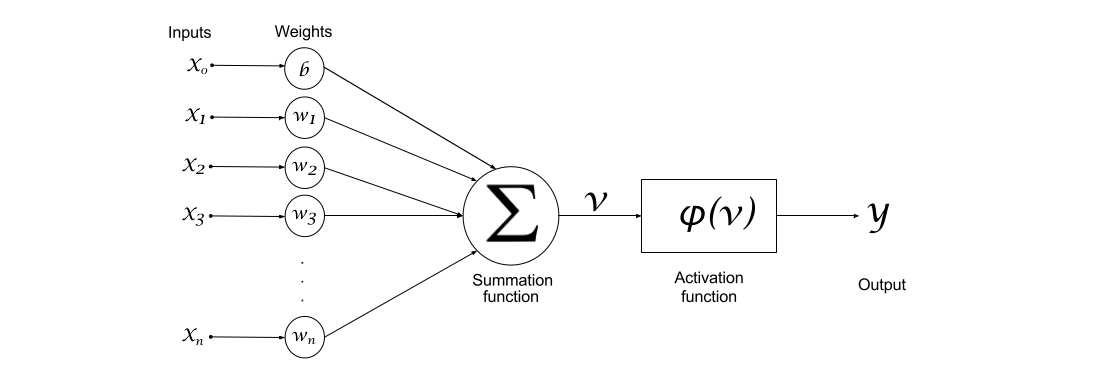
\includegraphics[scale=0.3]{images/aneuron.png}
        \caption{Artificial Neuron}
        \label{fig:31}
    \end{figure}
    
    \subsection{Non Linearity/ Activation Function}
    The capacity of the neural networks to approximate any functions, especially non-convex, is directly the result of the non-linear activation functions, referred as $\phi$ in the last section.  takes a vector and performs a certain fixed point-wise operation on it. There are three main activation functions:
    \vspace{5mm}
    \par \noindent
    \textbf{Sigmoid} The Sigmoid non-linearity has the following mathematical form:
    \begin{equation*}
        \phi=\sigma(x)=\frac{1}{1+e^{-x}}
    \end{equation*}
        It takes a real value and squashes it between 0 and 1. However, when the neuron's activation saturates at either tail of 0 or 1, the gradient at these regions is almost zero. Thus, the backpropagation algorithm fail at modifying its parameters and the parameters of the preceding neural layers.
    \vspace{5mm} \par \noindent
    \textbf{Hyperbolic Tangent} The TanH non-linearity has the following mathematical form
      \begin{equation*}
        \phi=2\sigma(2x)-1
    \end{equation*}
        It squashes a real-valued number between -1 and 1. However it has the same drawback as sigmoid.
    
    \vspace{5mm} \par \noindent
    \textbf{ReLU (Rectified Linear Unit)} The ReLU has the following mathematical form
    \begin{equation*}
        \phi=max(0,x)
    \end{equation*}
        The ReLU has become very popular in the last few years, because it was found to greatly
        accelerate the convergence of stochastic gradient descent compared to the sigmoid/tanh
        functions due to its linear non-saturating form. In fact, it does not suffer from the vanishing or exploding gradient. An other advantage is that it involves cheap operations compared to the expensive exponentials. However, the ReLU
        removes all the negative informations and thus appears not suited for all datasets and architectures.
    
    \subsection{Convolutional Layers}
    \subsubsection{Spatial Convolution Layer}
    Regular Neural Networks, only made of linear and activation layers, do not scale well to full images. For instance, images of size $3 \times 224 \times 224$ (3 color channels, 224 wide, 224 high) would necessitate a first linear layer having 3  $224 \times 224 + 1 = 150$, 129 parameters for a single neuron (e.g. output). Spatial convolution layers take advantage of the fact that their input (e.g. images or feature maps) exhibits many spatial relationships. In
    fact, neighboring pixels should not be affected by their location within image. Thus, a
    convolutional layer learns a set of $N_k$ filters $F = f_1 , ..., f_{N_k}$ , which are convolved spatially
    with input image $x$, to produce a set of $N_k$ 2D features maps $z$:
    
    \begin{equation*}
        z_k=f_k * x
    \end{equation*}
    
    where $*$ is the convolutional operator. When the filter correlates well with a region of the
    input image, the response in the corresponding feature map location is strong. Unlike
    conventional linear layer, weights are shared over the entire image reducing the number of
    parameters per response and equivariance is learned (i.e. an object shifted in the input image will simply shift the corresponding responses in a similar way). Also, a fully connected layer can be seen as a convolutional layer with filter of sizes $1 \times 1 \times inputSize$.  
    \par
    It is important to highlight that a spatial convolution is not defined by the spatial size
    of the input feature maps (e.g. wide and high), neither by the size of the output feature
    maps, but by the number of filters (e.g. number of output channels), the properties of its
    filters (e.g. number of input channels, wide, high) and the properties of the convolution
    (e.g. padding, stride).
    \begin{figure}[H]
        \centering
        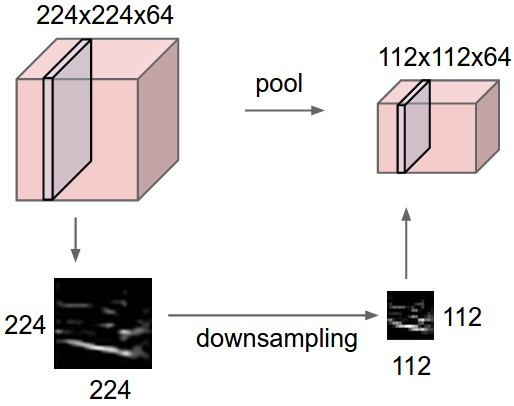
\includegraphics[scale=0.5]{images/spatialpooling.png}
        \caption[Spatial Pooling Operation]{The illustration of a spatial pooling operation in $2 \times 2$ regions by a stride of 2
        in the high direction, and 2 in the width direction, without padding.\cite{DBLP:journals/corr/CadeneTC16}}
        \label{fig:32}
    \end{figure}
    
    \subsubsection{Spatial Pooling}
            In Convolutional Neural Networks, a pooling layer is typically present to provide invariance
        to slightly different input images and to reduce the dimension of the feature maps (e.g.
        wide, high):
        \begin{equation*}
        p_R=P_{i \in R}(z_i)            
        \end{equation*}
        where $P$ is a pooling function over the region of pixels $R$. Max pooling is preferred as
        it avoids cancellation of negative elements and prevents blurring of the activations and
        gradients throughout the network since the gradient is placed in a single location during
        backpropagation.
        The spatial pooling layer is defined by its aggregation function, the high and width dimensions of the area where it is applied, and the properties of the convolution (e.g. padding,
        stride).
        
\section{Feed Forward Neural Networks}
    The most common architecture used in DNN is the \textit{Feed-Forward neural network}. Figure
    3 shows an example of a feed-forward neural network. In this framework, the neurons are
    arranged in layers. This architecture usually has three kinds of layers: an input layer, a few
    \textit{hidden layers} and an \textit{output layer}. The flow of information takes place from the input layer
    to the hidden layers and finally to the output layer which computes the final output. Each
    neuron in the different layers performs the same computation as shown in Equation \ref{eq:31} .
    \begin{figure}[H]
        \centering
        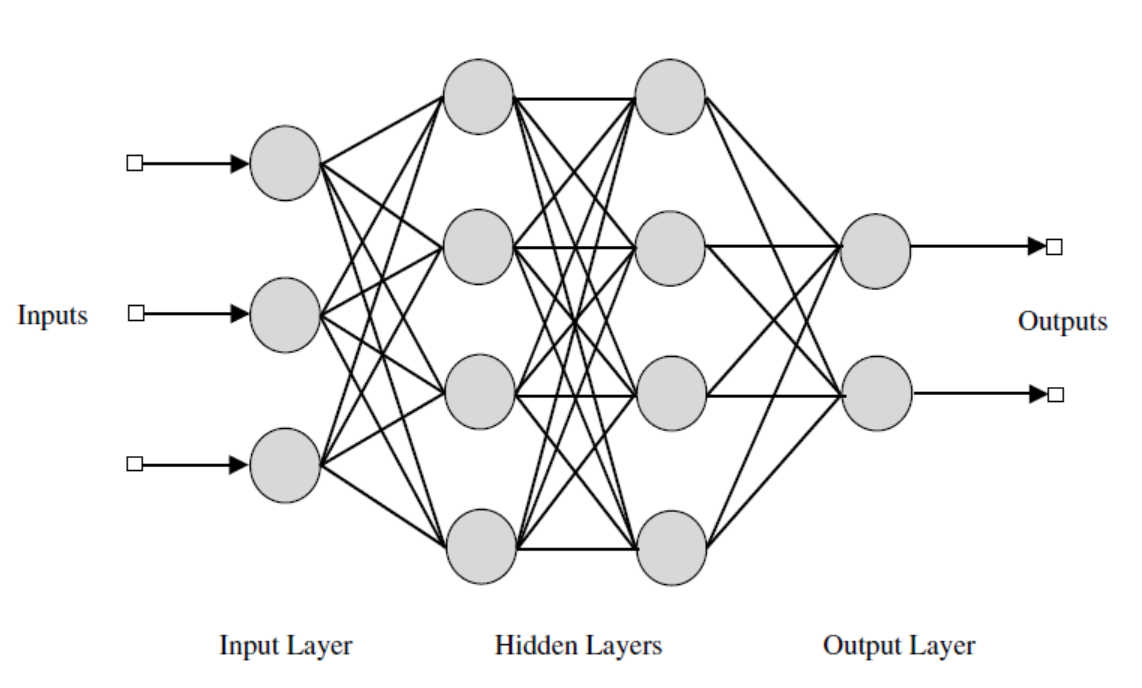
\includegraphics[scale=0.3]{images/ffnn.png}
        \caption[Feed Forward Neural Network]{Feed Forward Neural Network \cite{ffnn}}
        \label{fig:33}
    \end{figure}
    
\section{Deep Neural Networks}
        Traditional feedforward neural networks are considered to have the depth equal to the number of
    layers (i.e. the number of hidden layers plus 1, for the output layer). In many simple problems
    neural networks with depth 2 were successfully used, but there are many cases when single hidden
    layer is not enough. Solution to this problem is a deep neural network (DNN) - an artificial neural
    network with at least two hidden layers. The extra layers enable composition of features from
    lower layers, giving the potential of modeling complex, hierarchial features with a fewer units than
    in a shallow network. By providing sufficient amount of data to deep neural networks, it is often
    possible to learn better models than hand-coded features \cite{Krizhevsky:2012:ICD:2999134.2999257}.
    Before 2006 attempts at training deep architectures failed: training a deep feedforward neural network usually returns worse results than when using shallow architectures. Two papers \cite{Hinton:2006:FLA:1161603.1161605}\cite{Bengio:2006:GLT:2976456.2976476}, published in 2006, revolutionized deep architectures. The key principles in all
    of these papers were:
    \begin{itemize}
    \item unsupervised learning of representations is used to pre-train each layer,
    \item unsupervised training one layer at a time, using previously trained ones,
    \item supervised training to tune all layers together.
    \end{itemize}
    Deep neural networks are usually designed as basic feedforward networks, but in many recent
    studies deep learning architecture was created using convolutional deep neural networks (especially
    in image recognition and processing) \cite{DBLP:journals/corr/MnihKSGAWR13} \cite{mnih2015humanlevel}.
    
    \begin{figure}[H]
        \centering
        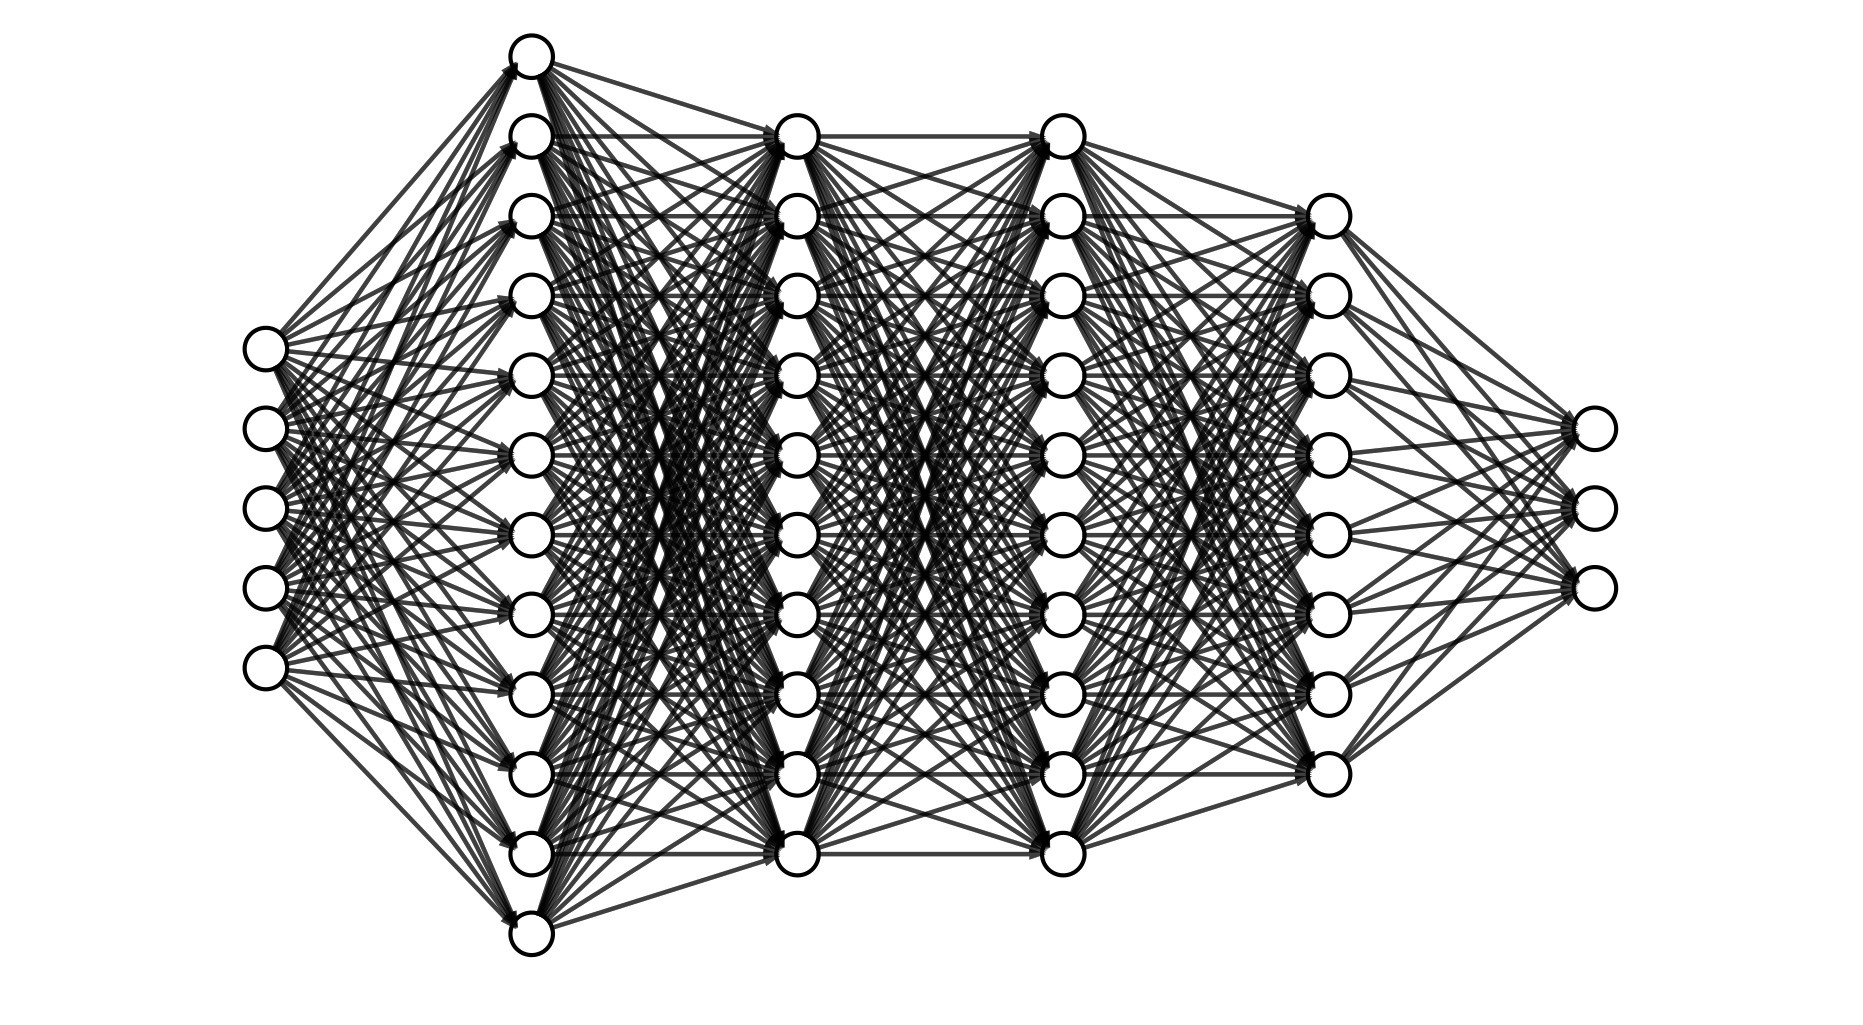
\includegraphics[scale=0.2]{images/dnn.png}
        \caption{Deep Neural Networks}
        \label{fig:34}
    \end{figure}
    
\section{Training Strategies/Methods}
    \subsection{Loss Function}
    To quantify the capacity of the network to approximate the ground truth
    labels for all training inputs, we define a loss function which takes as inputs the weights,
    biases, and examples from the training set. For instance, the loss could be the number
    of images correctly classified. Two most used loss functions to train deep neural networks are:
    
    \vspace{5mm}
    \par \noindent
    \textbf{Mean Squared Error (MSE)} MSE is a multi class loss formerly used to train neural
    networks.
    \begin{equation}
        Loss(x,y)= \frac{1}{n}\sum_i{|x_i-y_i|}^2
    \end{equation}
    with $x$ a vector of n predictions, and $y$ a binary vector full of 0 besides a 1 in the corresponding class dimension .
    
    \vspace{5mm}
    \par \noindent
    \textbf{Cross Entropy} Cross Entropy is a multi class loss which is nearly a better choice than MSE.
    \begin{equation}
        Loss(x,y)= -\sum_i y_i * log(\frac{e^{x_i}}{(\sum_j e^{x_j})})
    \end{equation}
    with $x$ a vector of n predictions, and $y$ a binary vector full of 0 besides a 1 in the corresponding class dimension .
   
    \subsection{Optimization}\label{sec:342}
    Once loss function for a neural network is decided, the training process is simply an (convex or non convex) optimization to minimize the value of the loss function. The idea in this approach is to start with a random initialization of the weights and calculate the output for a given input. the value of the loss function between the generated output and the actual output is used to update the weights of the network using an optimization algorithm. Since the weights are first updated of the output layer and then backpropagated into the network, the technique is known as \textit{backpropagation}.
    
    There are several optimization techniques commonly used in the training of neural networks, namely SGD (Stochastic Gradient Descent), Adagrad, RMSProp and Adam.
    
    The material on this subsection is taken from \cite{Goodfellow-et-al-2016}
    \subsubsection{Stochastic Gradient Descent (SGD)}
    Stochastic gradient descent (SGD) and its variants are probably the most used optimization algorithms for machine learning in general and for deep learning in particular. It is proven in  [Botton (1998)] that it is possible to obtain an unbiased estimate of the gradient by taking the average gradient on a minibatch of $m$ examples drawn i.i.d from the data-generating distribution.
    
        A crucial parameter for the SGD algorithm is the learning rate. Previously, we
    have described SGD as using a fixed learning rate $\epsilon$. In practice, it is necessary to
    gradually decrease the learning rate over time, so we now denote the learning rate
    at iteration $k$ as $\epsilon_k$ 
    This is because the SGD gradient estimator introduces a source of noise (the random sampling of
    $m$ training examples) that does not vanish even when we arrive at a minimum. By comparison, the true gradient of the total cost function becomes small and then
    become $0$ when we approach and reach a minimum using batch gradient descent, so batch gradient descent can use a fixed learning rate. A sufficient condition to guarantee convergence of SGD is that:
    
    \begin{equation}
        \sum_{k=1}^\infty \epsilon_k = \infty
    \end{equation}
    In practice, it is common to decay the learning rate linearly until iteration $\tau$:
    \begin{equation}
        \epsilon_k=(1-\alpha)\epsilon_0+\alpha \epsilon_\tau
    \end{equation}
    where $\alpha = \frac{k}{\tau}$. After iteration $\tau$, it is common to leave $\epsilon$ constant.
    The SGD algorithm is fully presented in Algorithm \ref{alg:2}:
 \vspace{5mm}
    \par
            \begin{algorithm}[H]\label{alg:2}
            \textbf{Require:} Learning Rate $\epsilon_1,\epsilon_2,...$ \\
            \textbf{Require:} Initial parameter $\theta$ \\
                $k \gets 1$ \\
                \While{stop condition not satisfied}{
                Sample a minibatch of $m$ examples from the training set {$x^{(i)},...x^{(m)}$} and corresponding targets $y^{(i)}$ \\
                Compute gradient estimate: $\hat{g} \gets \frac{1}{m} \nabla_\theta \sum_i L(f(x^{(i)};\theta),y^{(i)}) $ \\
                Apply update: $\theta \gets \theta- \epsilon_k \hat{g}$ \\
                $k\gets k+1$ \\
                }
            
            \caption{Stochastic Gradient Descent Update}
            \end{algorithm}

    
    
    \subsubsection{AdaGrad}
    The AdaGrad (Adaptive Gradient) algorithm, individually adapts the learning
    rates of all model parameters by scaling them inversely proportional to the square
    root of the sum of all the historical squared values of the gradient \cite{Duchi:2011:ASM:1953048.2021068}. 
    The parameters with the largest partial derivative of the loss have a
    correspondingly rapid decrease in their learning rate, while parameters with small
    partial derivatives have a relatively small decrease in their learning rate. The net
    effect is greater progress in the more gently sloped directions of parameter space.
    
        In the context of convex optimization, the AdaGrad algorithm enjoys some
    desirable theoretical properties. Empirically, however, for training deep neural
    network models, the accumulation of squared gradients from the \textit{beginning of
    training} can result in a premature and excessive decrease in the effective learning
    rate. AdaGrad performs well for some but not all deep learning models. AdaGrad algorithm is fully presented in Algorithm \ref{alg:3}:
 \vspace{5mm}
    \par
            \begin{algorithm}[H]\label{alg:3}
            \textbf{Require:} Learning Rate $\epsilon$ \\
            \textbf{Require:} Initial parameter $\theta$ \\
            \textbf{Require:} Small constant $\delta $ for numerical stability \\
                initialize gradient acculumation variable $r=0$ \\
                \While{stop condition not satisfied}{
                Sample a minibatch of $m$ examples from the training set {$x^{(i)},...x^{(m)}$} and corresponding targets $y^{(i)}$ \\
                Compute gradient estimate: $g \gets \frac{1}{m} \nabla_\theta \sum_i L(f(x^{(i)};\theta),y^{(i)}) $ \\
                Accumulate squared gradient: $r \gets r+g \bigodot g$ \\
                Compute update: $\Delta \theta \gets -\frac{\epsilon}{\delta+\sqrt{r}}\bigodot g.$ (Division and square root applied element-wise) \\
                Apply update: $\theta \gets \theta +\Delta \theta$\\

                }
            
            \caption{AdaGrad Update}
            \end{algorithm}

    
    
    \subsubsection{RMSProp}
    
        The RMSProp algorithm \cite{DBLP:journals/corr/abs-1207-0580} modifies AdaGrad to perform better in
    the nonconvex setting by changing the gradient accumulation into an exponentially
    weighted moving average. AdaGrad is designed to converge rapidly when applied to
    a convex function. When applied to a nonconvex function to train a neural network,
    the learning trajectory may pass through many different structures and eventually
    arrive at a region that is a locally convex bowl. AdaGrad shrinks the learning rate
    according to the entire history of the squared gradient and may have made the
    learning rate too small before arriving at such a convex structure. 
        RMSProp uses an exponentially decaying average to discard history from the extreme past so that
    it can converge rapidly after finding a convex bowl, as if it were an instance of the
    AdaGrad algorithm initialized within that bowl. RMSProp is shown in its standard form in Algorithm \ref{alg:4}:
 \vspace{5mm}
    \par
            \begin{algorithm}[H]\label{alg:4}
            \textbf{Require:} Learning Rate $\epsilon$, decay rate $\rho$ \\
            \textbf{Require:} Initial parameter $\theta$ \\
            \textbf{Require:} Small constant $\delta $ for numerical stability \\
                initialize gradient acculumation variable $r=0$ \\
                \While{stop condition not satisfied}{
                Sample a minibatch of $m$ examples from the training set {$x^{(i)},...x^{(m)}$} and corresponding targets $y^{(i)}$ \\
                Compute gradient estimate: $g \gets \frac{1}{m} \nabla_\theta \sum_i L(f(x^{(i)};\theta),y^{(i)}) $ \\
                Accumulate squared gradient: $r \gets \rho r+(1-\rho)g \bigodot g$ \\
                Compute update: $\Delta \theta \gets -\frac{\epsilon}{\delta+\sqrt{r}}\bigodot g.$ (Division and square root applied element-wise) \\
                Apply update: $\theta \gets \theta +\Delta \theta$\\

                }
            
            \caption{RMSProp Algorithm Update}
            \end{algorithm}

            
    \subsubsection{Adam}
        Adam \cite{DBLP:journals/corr/KingmaB14} is yet another adaptive learning rate optimization
        algorithm and is presented in Algorithm \ref{alg:5}. The name "Adam" derives from
        the phrase "adaptive moments". In the context of the earlier algorithms, it is
        perhaps best seen as a variant on the combination of RMSProp and momentum
        with a few important distinctions. First, in Adam, momentum is incorporated
        directly as an estimate of the first-order moment (with exponential weighting) of
        the gradient. The most straightforward way to add momentum to RMSProp is to
        apply momentum to the rescaled gradients. The use of momentum in combination
        with rescaling does not have a clear theoretical motivation. Second, Adam includes
        bias corrections to the estimates of both the first-order moments (the momentum
        term) and the (uncentered) second-order moments to account for their initialization
        at the origin. RMSProp also incorporates an estimate of the
        (uncentered) second-order moment; however, it lacks the correction factor. Thus,
        unlike in Adam, the RMSProp second-order moment estimate may have high bias
        early in training. Adam is generally regarded as being fairly robust to the choice
        of hyperparameters, though the learning rate sometimes needs to be changed from
        the suggested default.
         \vspace{5mm}
        \par
            \begin{algorithm}[H]\label{alg:5}
            \textbf{Require:} Step size $\epsilon$ \\
            \textbf{Require:} Initial parameter $\theta$ \\
            \textbf{Require:} Small constant $\delta $ for numerical stability \\
            \textbf{Require:} Exponential decay rate $\rho_1$ and $\rho_2$ (Suggested defaults: 0.9 and 0.999)
                initialize 1st and 2nd moment variables $s=0, r=0$ \\
                initialize time step t=0\\
                \While{stop condition not satisfied}{
                Sample a minibatch of $m$ examples from the training set {$x^{(i)},...x^{(m)}$} and corresponding targets $y^{(i)}$ \\
                Compute gradient estimate: $g \gets \frac{1}{m} \nabla_\theta \sum_i L(f(x^{(i)};\theta),y^{(i)}) $ \\
                $t \gets t+1$\\
                Update biased first moment estimate: $s \gets \rho_1 s+ (1-\rho_1)g$\\
                Update biased second moment estimate: $r \gets \rho_2 r+(1-\rho_2)g \bigodot g$\\
                Correct bias in first moment: $\hat{s} \gets \frac{s}{1-\rho_1^t}$\\
                Correct bias in second moment: $\hat{r} \gets \frac{r}{1-\rho_2^t}$\\
                Compute update: $\Delta \theta \gets -\frac{\epsilon}{\delta+\sqrt{r}}\bigodot g.$ (Division and square root applied element-wise) \\
                Apply update: $\theta \gets \theta +\Delta \theta$\\

                }
            
            \caption{The Adam algorithm}
            \end{algorithm}

\section{Deep Q-learning}
    \label{sec:dql}
    $Q$-learning (Section \ref{sec:253}) has been a widely used algorithm for model-free reinforcement learning. However, reinforcement learning is known to be unstable (or even to diverge) when a nonlinear function approximator such as a neural network is used to represent the Q-function \cite{Tsitsiklis97ananalysis}. This instability is caused by correlations between succeeding observations, the fact, that small updates of $Q$-function
    may substantially change policy, and the correlations between the $Q$-value and target values. There's a breakthrough for this problem, proposed by \cite{mnih2015humanlevel}, it was shown that $Q$-learning could be used with Deep Neural Networks and the algorithm showed human level performance on seven Atari 2600 games using only raw image pixels as the input. The key points of this paper is an mechanism called \textit{experience replay}.
    \par
    \subsection{Experience Replay and Minibatches Learning}
         To inhibit first of this issues, biologically-inspired mechanism called experience
        replay is used \cite{Lin1992}. In this idea, the agent can experience the effects of its actions without actually executing them. Data used to learning is randomly sampled at each step from memory of agent's previous transitions, what removes the correlation in the sequence of training examples and smooths the training distribution over many past behaviors, thus reducing oscillations and divergence of the learning process. Another advantage of this mechanism is reusing single experience in many weights updates, which allows for greater data efficiency \cite{mnih2015humanlevel}. Note that using experience replay implies
        off-policy learning (see Section \ref{sec:253}), because current parameters are different than the ones used to generate experience sample. 
    \par
         To perform experience replay, agent's transitions experience at each time step t are stored in dataset $D$ as a tuple $ e_t = (s_t , a_t , r_t , s_t+1 , i_t+1 )$, where $s_t$ is state observed at time $t$, $a_t$ is action
        performed after observing state $s_t$ , $r_t$ is reward given for executing action $a_t$ , $s_t+1$ is resulting
        state after taking action $a_t$ , and $i_t+1$ stores information if state $s_t+1$ is terminal. The dataset (also
        called, replay memory) $D_N = {e_1 , e_2 , ..., e_n }$ stores last $N$ experience tuples.
    \par
        Another technique, used tightly together with experience replay, is \textit{minibatch learning}, which consists in, basically, learning more than one training example at each step. It can perform significantly more efficient than standard, single-sample stochastic gradient descent methods because the code can make use of vectorization libraries or GPU rather than computing each step separately.
    \par
        This makes the learning process also less prone to outliers and noises, as the gradient computed at each step uses more training examples. Generally, determining the gradient of a batch involves computing cost function over each training example in the batch and then, at the end, summing the results of these functions. When planning the size of the minibatch, some trade-offs between efficiency and noisiness have to be made: small size of the minibatch is more susceptible to noise (which may lead to stagnation in local optimum), whereas with large size of the minibatch, the up- date of single parameter will last longer. Moreover, too large minibatch may end up with bouncing around a local optimum instead of converging to one.
        \par
        At each step of the training, dataset $D$ is sampled uniformly at random to get minibatch of experiences of size $M (( s, a, r, s' , i) \sim U (D))$ and perform learning (weights updates) on them. This solution is, however, limited because the memory does not differentiate important experiences from insignificant ones and always overwrites the oldest transition with the most recent one. Similarly, the uniform sampling gives equal importance to all of the transitions. Full pseudocode of Deep $Q$-Learning algorithm with experience replay and minibatches is presented in Algorithm \ref{alg:6}:
 \vspace{5mm}
        \par
            \begin{algorithm}[H]\label{alg:6}
            
            \textbf{Require:} Replay memory $D$ with capacity $N$ \\
            \textbf{Require:} Initial parameter $\theta_0$ \\
            \ForEach{episode $e$, unless stop condition satisfied}
                {
                Get initial state $s_0$ \\
               
               \ForEach{timestep $t$ in current episode $e$}
                    {
                       Using $\epsilon$-greedy policy, select action $a_t$\\
                       Execute action $a_t$\\
                       Observe following state $s_{t+1}$ and whether it is terminal ($i_{t+1}$)\\
                       Store transition $(s_t,r_t,a_t,s_{t+1},i_{t+1})$\\
                       Sample random minibatch of transitions $(s_j,r_j,a_j,s_{j+1},i_{j+1})$   of size $M$ from $D$\\
                       \ForEach{sample in the minibatch}
                            {
                                \eIf{$i_j+1$ is true}{$y_j=r_j$}
                                {$y_j=r_j+\gamma \max_{a'}Q(s_{j+1},a',\theta)$}
                            }
                    }
                    Perform backpropagation algorithm with optimizer explained in Section \ref{sec:342} \\
                }

            \caption{Deep $Q$-learning with experience replay}
            \end{algorithm}
            
    \subsection{Target Network Freezing}
    Another modification of the standard $Q$-learning aimed to further improve its when using neural networks is freezing weights of the target $Q$-network \cite{mnih2015humanlevel}. More precisely, there are two separated networks maintained:
    \begin{enumerate}
        \item
        A target network, called $\hat{Q}$ in the following, with fixed set of old parameters $\theta^-$ for generating $Q$ values, used in $Q$-learning process.
        \item A network for interacting with the environment (generating $Q$-values for each possible action in current state), with the current set of parameters $\theta$.
    \end{enumerate}
    
        At every update iteration, the current parameters $\theta$ are updated to minimize the w.r.t the old parameters $\theta^-$ by optimizing the Loss function for $\theta$, an example of this would be using the \textbf{MSE} loss function, which resulted in the following loss function:
        \begin{equation}\label{eq:36}
            L(\theta)=\E_{s,a,r,s',i \sim D}[(R(s,a)+\gamma max_{a'}\hat{Q}(s',a',\theta^-)-Q(s,a,\theta))^2]
        \end{equation}
        
        
        Every $C$ steps, parameters from the $Q$-network are copied to the target $Q$-network ($\theta^- \gets \theta$)
        Generating the learning targets using an older set of weights adds a delay between the time an update to $Q$ is made and the time the update affects the targets, counteracting oscillations and divergence.
        
        	\section{Literature Review}
        	In the early days of machine learning, most of the approach used to solve problems are either supervised or unsupervised learning. This two machine learning methods are considered reliable because they are generally well-defined. Reinforcement learning, on the other hand, is generally avoided because of no formal and proven method to solve any problems with reinforcement learning. Reinforcement learning algorithm are considered \textit{hit or miss} because of the '\textit{trial and error}' nature of reinforcement learning. It was until Watkins et al. \cite{Watkins:1989} developed the $Q$-learning algorithm, a formal, iterative and proven method using value function iteration. This $Q$-learning algorithm changes reinforcement learning forever, as this is still the most used reinforcement learning algorithm until today.
            \par
            Despite being a huge success, the advances of reinforcement learning, or even the field of machine learning in general was kinda stagnant around that era (1990s). The main reason being the computational power to facilitate the training wasn't there yet. Not to mention, almost any machine learning algorithm are generally not useful unless it's properly trained with a lot of data. Artificial neural networks, which was the trending topic around (1990s) tries to help solving some of the machine learning tasks, albeit the result was still lacking. Bottou et al. \cite{Bottou2010} finally solved this problem on 2010 by introducing Stochastic Gradient Descent (SGD) or minibatch Gradient Descent. Stochastic Gradient Descent allows for training in large-scale problems using the fact that it trains the neural network (update parameters) batch-by-batch. This rather simple-looking allows neural networks to be updated more frequently, while still reflects the training data. A neural network that requires huge amount of data now has a much higher convergence rate. because of the smaller, but better steps that the gradient update takes throughout the iteration.
            \par
            SGD completely revolutionize the world of artificial neural networks. Neural networks plays a huge role in the huge popularity explosion of machine learning in 2010s. Deep neural networks (DNN) soon emerge as a multi-layer extension of neural networks. However, the first major achievement of deep neural networks is on 2012, when Krizhevsky et al. developed an image classification/recognition framework called ImageNet \cite{Krizhevsky:2012:ICD:2999134.2999257}. ImageNet soon become the pinnacle of image recognition, and pushes deep learning to become a major subfield of machine learning. Which become even more popular nowadays. 
            In 2013 DeepMind, an artificial intelligence company which was recently acquired by Google, released a paper called Playing Atari with Deep Reinforcement Learning \cite{DBLP:journals/corr/MnihKSGAWR13}. In this paper an agent was trained to play various Atari games, On 20 of the 49 games the
            agent outperformed the average human player. What is even more astonishing, is the fact that the only
            input the system received was the visual input,using the similar deep CNN used by ImageNet \cite{Krizhevsky:2012:ICD:2999134.2999257} and the received amount of points.  The goal of the game,
            nor the actual influence of each action on the environment were programmed into the system. This was
            all learned along the path. In fact, this is also the information that is available when a human learns such a
            game. 
            \par
            On a later date the same group of researchers published a more technical report concerning these
            findings, titled "Human-level Control through Deep Reinforcement Learning" \cite{mnih2015humanlevel}.
            To achieve all this, a new algorithm called Deep $Q$-Learning (DQL) was developed. DQL is a deep RL
            technique that combines two highly popular machine learning techniques, Q-learning and Convolutional
            Neural Networks (CNNs). The former is one of the most frequently used algorithms to solve RL problems.
            The technique uses a $Q$-function that attributes a value to each action in every possible state. The latter is
            a deep learning technique, which gained much traction in recent years. CNNs are especially known for
            their capabilities to deal with raw images as input. DeepMind successfully solved the long-standing problem of combining $Q$-learning with deep neural networks, which is the instability of the neural network approximation to $Q$-function. In DQL, a CNN is used as a function approximator for the Q-function. In this context the used CNN is often referred to as the Deep $Q$-Network (DQN).
                
           \par
            The newly developed technique of DQL opens many new research opportunities. It is a big step forward towards introducing RL to more realistic contexts. The current achievements of this technique are remarkably promising, which indicates that this technique can be applied to various other RL problems besides the simple and basic atari games.
            \par
            
            Two years later, again, the same researcher from DeepMind found a problem with the Q-learning algorithm. It often overestimates the action values because it uses the same value function for action-selection and action-evaluation. To solve this, DeepMind developed double DQN, that is based on double $Q$-learning \cite{DBLP:journals/corr/HasseltGS15}, that reduces the observed overestimation by learning two value networks 0 with parameters $\theta$ and $\theta^-$ that both use the other network for value-estimation. This technique shows major improvements in network stability and since then has been widely used in deep-reinforcement learning community, because big the difference is despite the small amount of change that is needed to be implemented.
            
            However, DeepMind's method still suffers from the fact that when the game gets more and more complex, the computational time needed grows exponentially. Not only that, most of the time, the deep $Q$-network either diverges or oscillates around the target minima. This was actually a well-known problem because Stochastic Gradient Descent and RMSProp, used in DQN have a tendency to diverge in certain situations. In order to solve this, Kingma et al. \cite{DBLP:journals/corr/KingmaB14} developed an adaptive gradient optimizer called Adam. Adam uses first 2 moments (the average and uncentered variance) to scale the gradient. This allows Adam to deal with sparse-gradient and non-stationary objectives.
            
            The outline of this literature review can be seen on Table \ref{tab:31}:
            \begin{table}[H]
                \centering
                
                \begin{tabularx}{\linewidth}{|>{\hsize=.1\hsize \setlength{\baselineskip}{0.75\baselineskip}}X|>{\hsize=0.8\hsize \setlength{\baselineskip}{0.75\baselineskip}}X|>{\hsize=1.5\hsize \setlength{\baselineskip}{0.75\baselineskip}}X|>{\hsize=1.6\hsize \setlength{\baselineskip}{0.75\baselineskip}}X|}
                    \hline
                     & Authors & Topic & Result \\
                     \hline
                     1. & Chris Watkins & Learning from delayed rewards & $Q$-Learning\\
                     2. & Leon Bottou & Large Scale Machine Learning with Stochastic Gradient Descent & Stochastic Gradient Descent, a training method for huge datasets\\
                     3. & Krizhevsky et al. & ImageNet Classification with Deep Convolutional Neural Networks & Deep Convolutional Neural Network for Image Classification\\ 
                     4. & Mnih et al. & Human Level Control through Deep Reinforcement Learning & Deep $Q$-Network and Deep $Q$-Learning\\
                     5. & Hasselt et al. & Deep Reinforcement Learning with Double $Q$-learning & Double Deep $Q$-Learning and Target Network Freezing\\
                     6. & Kingma et al. & Adam: a method for stochastic optimization & Adam optimizer for neural network training \\
                     \hline
                \end{tabularx}
                \caption{Outline of Literature Review}
                \label{tab:31}
            \end{table}